\documentclass[a4paper, 12pt]{article}

\usepackage[utf8]{inputenc}
\usepackage[T1, T2A]{fontenc}
\usepackage[english, russian]{babel}
\usepackage[top=2cm, left=2cm, right=2cm, bottom=2cm]{geometry}

%%% Visualization
\usepackage{graphics, subcaption, graphicx}

%%% Text
\usepackage{pscyr, indentfirst, enumitem}

%%% Tables
\usepackage{tabu, booktabs}

%%% Math
\usepackage{amsmath,amssymb,amsthm,bm,mathtools}
\newcommand{\diff}{\text{d}}      % Fourier transform operator

\begin{document}

\begin{figure}
    \centering
    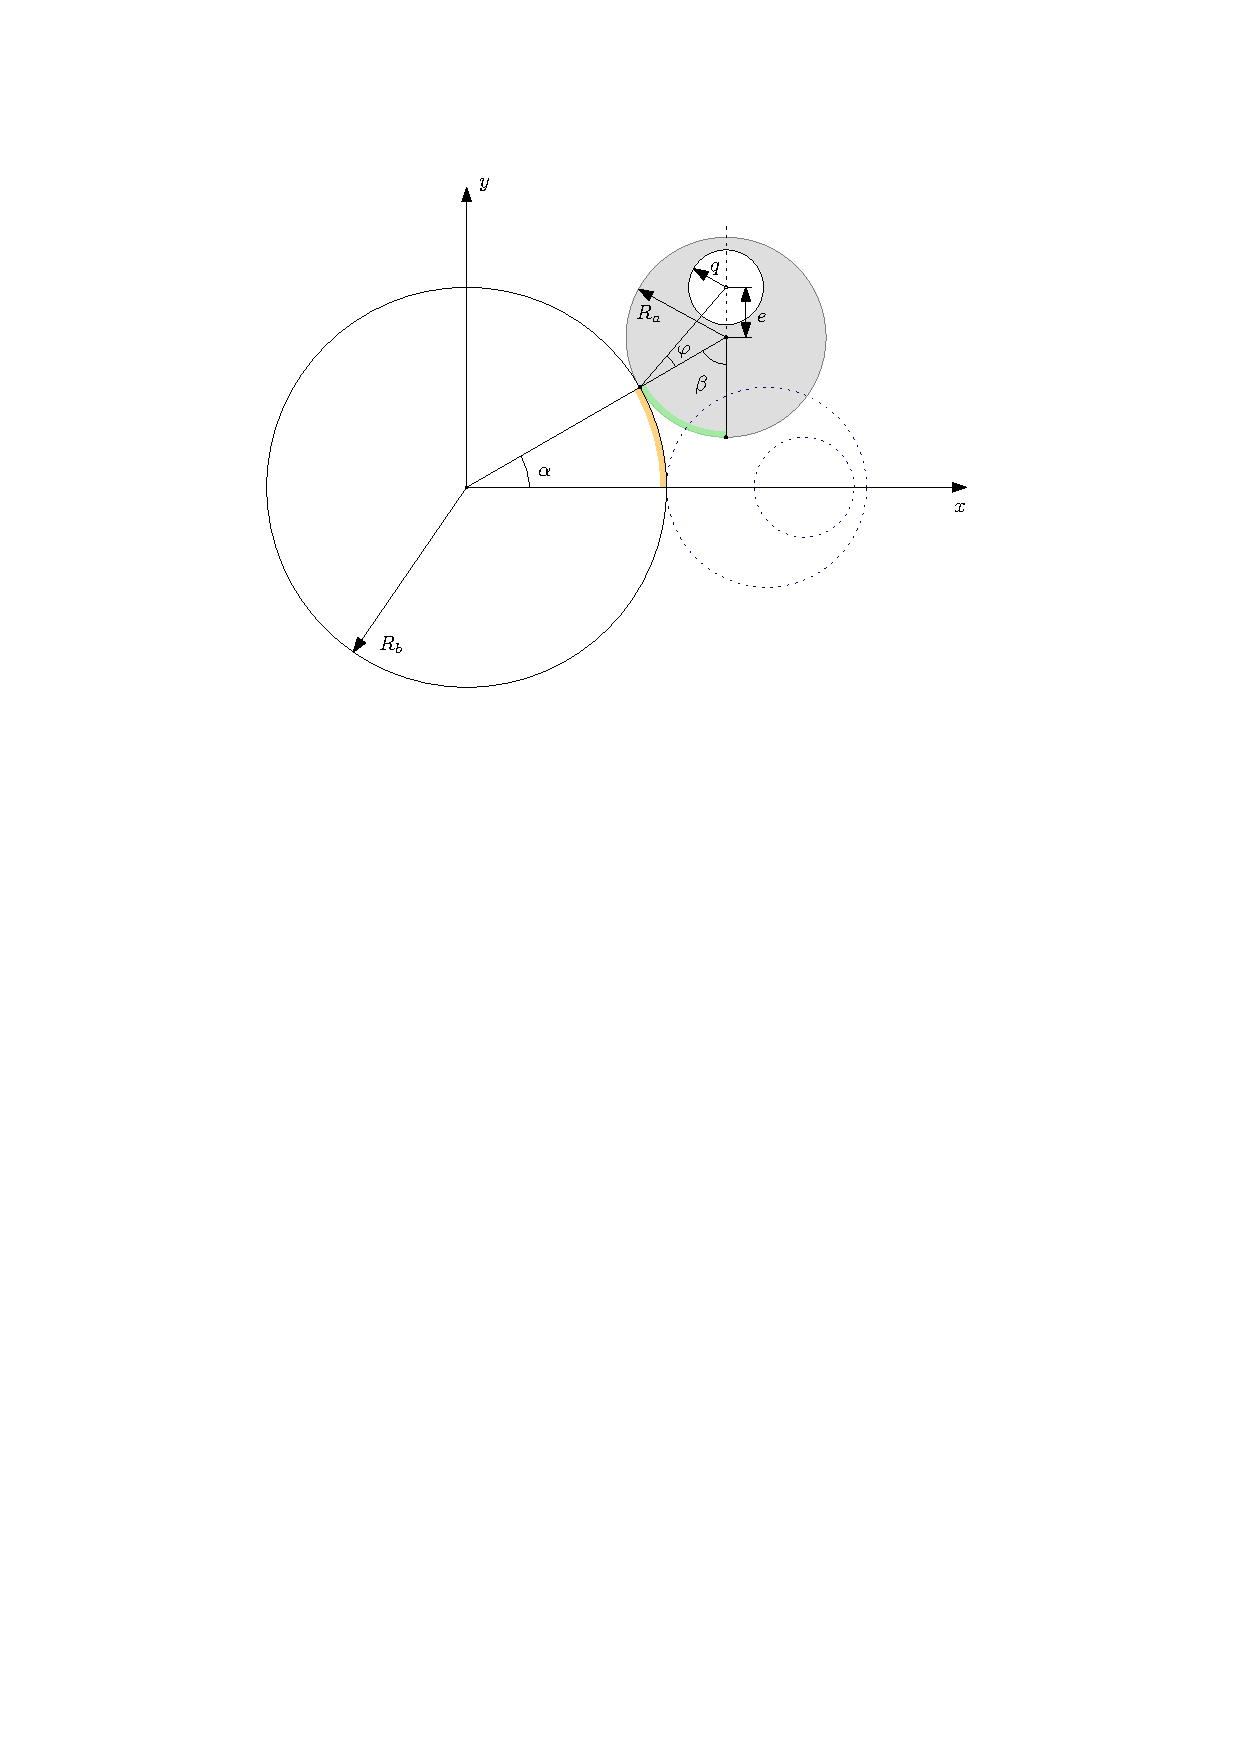
\includegraphics{images/Profile-description1.pdf}
\end{figure}

Траектория профиля описывается варежения для трехзвенного механизма:
\begin{equation}
    \begin{split}
        x_p & = (R_b + R_a)\cos{(\alpha)} + e\cos{(\alpha + \beta)} - q\cos{(\alpha + \varphi)} \\
        y_p & = (R_b + R_a)\sin{(\alpha)} + e\sin{(\alpha + \beta)} - q\sin{(\alpha + \varphi)}
    \end{split}
\end{equation}
здесь углы $\bm{\beta}$ и $\bm{\varphi}$ определяются по формулам:
\begin{align}
    \beta &= \frac{R_b}{R_a}\alpha \\
    \tan{\varphi} &= \frac{\sin{(\beta)}}{\frac{R_a}{e} + \cos{(\beta)}}
\end{align}

Число зубьев определяется по формуле:
\begin{equation}
    \alpha_{max} = \frac{R_a}{R_b}2\pi \rightarrow z_1 = \frac{2\pi}{\alpha_{max}} = \frac{R_b}{R_a}
\end{equation}
    
Примем $\bm{R_a} = \frac{m}{2}$, тогда получаем удобную параметризацию:
\begin{align}
    R_a & = \frac{m}{2} \\
    R_b & = R_a z_1 \\
    q   & = m \\
    e_0 & = \frac{m}{2} \\
    e   & = x \frac{m}{2}
\end{align}

С учет данных, получим некоторые параметры зубчатого колеса.

Радиус циклоиды:
\begin{equation}
    \begin{split}
        r_1 & = R_a + R_b + e - q = \frac{R_b}{z_1} + R_b + x\frac{m}{2} - 2\frac{m}{2} \\
            & = \frac{R_b}{z_1} + R_b + x\frac{R_b}{z_1} - 2 \frac{R_b}{z_1} = R_b \frac{1+z_1+x-2}{z_1} = R_b + R_b\frac{x-1}{z_1}
    \end{split}
\end{equation}

\end{document}
